% Options for packages loaded elsewhere
\PassOptionsToPackage{unicode}{hyperref}
\PassOptionsToPackage{hyphens}{url}
%
\documentclass[
]{article}
\usepackage{lmodern}
\usepackage{amssymb,amsmath}
\usepackage{ifxetex,ifluatex}
\ifnum 0\ifxetex 1\fi\ifluatex 1\fi=0 % if pdftex
  \usepackage[T1]{fontenc}
  \usepackage[utf8]{inputenc}
  \usepackage{textcomp} % provide euro and other symbols
\else % if luatex or xetex
  \usepackage{unicode-math}
  \defaultfontfeatures{Scale=MatchLowercase}
  \defaultfontfeatures[\rmfamily]{Ligatures=TeX,Scale=1}
\fi
% Use upquote if available, for straight quotes in verbatim environments
\IfFileExists{upquote.sty}{\usepackage{upquote}}{}
\IfFileExists{microtype.sty}{% use microtype if available
  \usepackage[]{microtype}
  \UseMicrotypeSet[protrusion]{basicmath} % disable protrusion for tt fonts
}{}
\makeatletter
\@ifundefined{KOMAClassName}{% if non-KOMA class
  \IfFileExists{parskip.sty}{%
    \usepackage{parskip}
  }{% else
    \setlength{\parindent}{0pt}
    \setlength{\parskip}{6pt plus 2pt minus 1pt}}
}{% if KOMA class
  \KOMAoptions{parskip=half}}
\makeatother
\usepackage{xcolor}
\IfFileExists{xurl.sty}{\usepackage{xurl}}{} % add URL line breaks if available
\IfFileExists{bookmark.sty}{\usepackage{bookmark}}{\usepackage{hyperref}}
\hypersetup{
  pdftitle={MM2-eksamen},
  pdfauthor={Mads Hovaldt},
  hidelinks,
  pdfcreator={LaTeX via pandoc}}
\urlstyle{same} % disable monospaced font for URLs
\usepackage[margin=1in]{geometry}
\usepackage{color}
\usepackage{fancyvrb}
\newcommand{\VerbBar}{|}
\newcommand{\VERB}{\Verb[commandchars=\\\{\}]}
\DefineVerbatimEnvironment{Highlighting}{Verbatim}{commandchars=\\\{\}}
% Add ',fontsize=\small' for more characters per line
\usepackage{framed}
\definecolor{shadecolor}{RGB}{248,248,248}
\newenvironment{Shaded}{\begin{snugshade}}{\end{snugshade}}
\newcommand{\AlertTok}[1]{\textcolor[rgb]{0.94,0.16,0.16}{#1}}
\newcommand{\AnnotationTok}[1]{\textcolor[rgb]{0.56,0.35,0.01}{\textbf{\textit{#1}}}}
\newcommand{\AttributeTok}[1]{\textcolor[rgb]{0.77,0.63,0.00}{#1}}
\newcommand{\BaseNTok}[1]{\textcolor[rgb]{0.00,0.00,0.81}{#1}}
\newcommand{\BuiltInTok}[1]{#1}
\newcommand{\CharTok}[1]{\textcolor[rgb]{0.31,0.60,0.02}{#1}}
\newcommand{\CommentTok}[1]{\textcolor[rgb]{0.56,0.35,0.01}{\textit{#1}}}
\newcommand{\CommentVarTok}[1]{\textcolor[rgb]{0.56,0.35,0.01}{\textbf{\textit{#1}}}}
\newcommand{\ConstantTok}[1]{\textcolor[rgb]{0.00,0.00,0.00}{#1}}
\newcommand{\ControlFlowTok}[1]{\textcolor[rgb]{0.13,0.29,0.53}{\textbf{#1}}}
\newcommand{\DataTypeTok}[1]{\textcolor[rgb]{0.13,0.29,0.53}{#1}}
\newcommand{\DecValTok}[1]{\textcolor[rgb]{0.00,0.00,0.81}{#1}}
\newcommand{\DocumentationTok}[1]{\textcolor[rgb]{0.56,0.35,0.01}{\textbf{\textit{#1}}}}
\newcommand{\ErrorTok}[1]{\textcolor[rgb]{0.64,0.00,0.00}{\textbf{#1}}}
\newcommand{\ExtensionTok}[1]{#1}
\newcommand{\FloatTok}[1]{\textcolor[rgb]{0.00,0.00,0.81}{#1}}
\newcommand{\FunctionTok}[1]{\textcolor[rgb]{0.00,0.00,0.00}{#1}}
\newcommand{\ImportTok}[1]{#1}
\newcommand{\InformationTok}[1]{\textcolor[rgb]{0.56,0.35,0.01}{\textbf{\textit{#1}}}}
\newcommand{\KeywordTok}[1]{\textcolor[rgb]{0.13,0.29,0.53}{\textbf{#1}}}
\newcommand{\NormalTok}[1]{#1}
\newcommand{\OperatorTok}[1]{\textcolor[rgb]{0.81,0.36,0.00}{\textbf{#1}}}
\newcommand{\OtherTok}[1]{\textcolor[rgb]{0.56,0.35,0.01}{#1}}
\newcommand{\PreprocessorTok}[1]{\textcolor[rgb]{0.56,0.35,0.01}{\textit{#1}}}
\newcommand{\RegionMarkerTok}[1]{#1}
\newcommand{\SpecialCharTok}[1]{\textcolor[rgb]{0.00,0.00,0.00}{#1}}
\newcommand{\SpecialStringTok}[1]{\textcolor[rgb]{0.31,0.60,0.02}{#1}}
\newcommand{\StringTok}[1]{\textcolor[rgb]{0.31,0.60,0.02}{#1}}
\newcommand{\VariableTok}[1]{\textcolor[rgb]{0.00,0.00,0.00}{#1}}
\newcommand{\VerbatimStringTok}[1]{\textcolor[rgb]{0.31,0.60,0.02}{#1}}
\newcommand{\WarningTok}[1]{\textcolor[rgb]{0.56,0.35,0.01}{\textbf{\textit{#1}}}}
\usepackage{graphicx,grffile}
\makeatletter
\def\maxwidth{\ifdim\Gin@nat@width>\linewidth\linewidth\else\Gin@nat@width\fi}
\def\maxheight{\ifdim\Gin@nat@height>\textheight\textheight\else\Gin@nat@height\fi}
\makeatother
% Scale images if necessary, so that they will not overflow the page
% margins by default, and it is still possible to overwrite the defaults
% using explicit options in \includegraphics[width, height, ...]{}
\setkeys{Gin}{width=\maxwidth,height=\maxheight,keepaspectratio}
% Set default figure placement to htbp
\makeatletter
\def\fps@figure{htbp}
\makeatother
\setlength{\emergencystretch}{3em} % prevent overfull lines
\providecommand{\tightlist}{%
  \setlength{\itemsep}{0pt}\setlength{\parskip}{0pt}}
\setcounter{secnumdepth}{-\maxdimen} % remove section numbering

\title{MM2-eksamen}
\author{Mads Hovaldt}
\date{28/10/2020}

\begin{document}
\maketitle

We have the dataset ChestSim1000

\begin{Shaded}
\begin{Highlighting}[]
\KeywordTok{data}\NormalTok{(chestSim1000, }\DataTypeTok{package=}\StringTok{"gRbase"}\NormalTok{)}
\KeywordTok{head}\NormalTok{(chestSim1000)}
\end{Highlighting}
\end{Shaded}

\begin{verbatim}
##   asia tub smoke lung bronc either xray dysp
## 1   no  no    no   no   yes     no   no  yes
## 2   no  no   yes   no   yes     no   no  yes
## 3   no  no   yes   no    no     no   no   no
## 4   no  no    no   no    no     no   no   no
## 5   no  no   yes   no   yes     no   no  yes
## 6   no  no   yes  yes   yes    yes  yes  yes
\end{verbatim}

This is a hyphotetical Chest Clinic problem, by Lauritzen and
Spiegelhalter. (ref til \url{https://arxiv.org/pdf/1301.7394.pdf})

Here is a short explanation of the variables in the dataset.

\begin{itemize}
\tightlist
\item
  asia \(\rightarrow\) subject has visited asia
\item
  tub \(\rightarrow\) subject has tuberculosis
\item
  smoke \(\rightarrow\) subject is a smoker
\item
  lung \(\rightarrow\) subject has lung cancer
\item
  bronc \(\rightarrow\) subject has bronchitis
\item
  either \(\rightarrow\) subject has either tuberculosis or lungcancer
\item
  xray \(\rightarrow\) subject has positive X-ray
\item
  dysp \(\rightarrow\) Subject has dyspnoea
\end{itemize}

Shortness-of-breath (dyspnoea) may be due to tuberculosis, lung cancer,
bronchitis, none of them, or more than one of them. A recent visit to
Asia increases the chances of tuberculosis, while smoking is known to be
a risk factor for both lung cancer and bronchitis. The results of a
single chest X-ray do not discriminate between lung cancer and
tuberculosis, as does neither the presence nor absence of dyspnoea.
(citat direkte sat ind fra \url{https://arxiv.org/pdf/1301.7394.pdf})

\begin{Shaded}
\begin{Highlighting}[]
\NormalTok{dg1 <-}\StringTok{ }\KeywordTok{dag}\NormalTok{(}\OperatorTok{~}\StringTok{ }\NormalTok{S }\OperatorTok{+}\StringTok{ }\NormalTok{L}\OperatorTok{|}\NormalTok{S }\OperatorTok{+}\StringTok{ }\NormalTok{X}\OperatorTok{|}\NormalTok{L}\OperatorTok{:}\NormalTok{S }\OperatorTok{+}\StringTok{ }\NormalTok{B}\OperatorTok{|}\NormalTok{S }\OperatorTok{+}\StringTok{ }\NormalTok{D}\OperatorTok{|}\NormalTok{L}\OperatorTok{:}\NormalTok{B)}
\KeywordTok{plot}\NormalTok{(dg1)}
\end{Highlighting}
\end{Shaded}

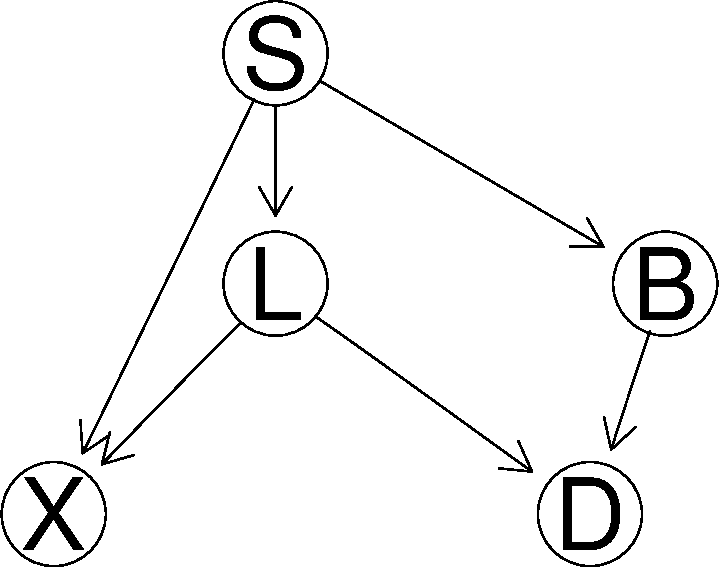
\includegraphics{PresentationDel1_files/figure-latex/unnamed-chunk-3-1.pdf}

\begin{Shaded}
\begin{Highlighting}[]
\NormalTok{dg2<-}\KeywordTok{dag}\NormalTok{(}\OperatorTok{~}\StringTok{ }\NormalTok{asia}\OperatorTok{+}\NormalTok{tub}\OperatorTok{|}\NormalTok{asia}\OperatorTok{+}\StringTok{ }\NormalTok{either}\OperatorTok{|}\NormalTok{tub}\OperatorTok{:}\NormalTok{lung}\OperatorTok{+}\NormalTok{smoke}\OperatorTok{+}\NormalTok{lung}\OperatorTok{|}\NormalTok{smoke}\OperatorTok{+}\NormalTok{bronc}\OperatorTok{|}\NormalTok{smoke}\OperatorTok{+}\NormalTok{dysp}\OperatorTok{|}\NormalTok{either}\OperatorTok{:}\NormalTok{bronc}\OperatorTok{+}\NormalTok{xray}\OperatorTok{|}\NormalTok{either)}
\KeywordTok{plot}\NormalTok{(dg2)}
\end{Highlighting}
\end{Shaded}

\includegraphics{PresentationDel1_files/figure-latex/unnamed-chunk-4-1.pdf}

\hypertarget{opgave-1}{%
\section{Opgave 1}\label{opgave-1}}

\begin{Shaded}
\begin{Highlighting}[]
\NormalTok{Counting1 <-}\StringTok{ }\ControlFlowTok{function}\NormalTok{(x,y,z)\{ }\CommentTok{#counting the number of observation for x and y}
 \ControlFlowTok{if}\NormalTok{ (x}\OperatorTok{!=}\DecValTok{0} \OperatorTok{&&}\StringTok{ }\NormalTok{y}\OperatorTok{!=}\DecValTok{0} \OperatorTok{&&}\StringTok{ }\NormalTok{z}\OperatorTok{==}\DecValTok{0}\NormalTok{)\{}
\NormalTok{  a11 <-}\StringTok{ }\NormalTok{(}\KeywordTok{length}\NormalTok{(}\KeywordTok{which}\NormalTok{(chestSim1000[x]  }\OperatorTok{==}\StringTok{ "yes"} \OperatorTok{&}\StringTok{ }\NormalTok{chestSim1000[y] }\OperatorTok{==}\StringTok{ "yes"}\NormalTok{)))}
\NormalTok{  a12 <-}\StringTok{ }\NormalTok{(}\KeywordTok{length}\NormalTok{(}\KeywordTok{which}\NormalTok{(chestSim1000[x] }\OperatorTok{==}\StringTok{ "no"} \OperatorTok{&}\StringTok{ }\NormalTok{chestSim1000[y] }\OperatorTok{==}\StringTok{ "yes"}\NormalTok{)))}
\NormalTok{  a21 <-}\StringTok{ }\NormalTok{(}\KeywordTok{length}\NormalTok{(}\KeywordTok{which}\NormalTok{(chestSim1000[x] }\OperatorTok{==}\StringTok{ "yes"} \OperatorTok{&}\StringTok{ }\NormalTok{chestSim1000[y] }\OperatorTok{==}\StringTok{ "no"}\NormalTok{)))}
\NormalTok{  a22 <-}\StringTok{ }\NormalTok{(}\KeywordTok{length}\NormalTok{(}\KeywordTok{which}\NormalTok{(chestSim1000[x] }\OperatorTok{==}\StringTok{ "no"} \OperatorTok{&}\StringTok{ }\NormalTok{chestSim1000[y] }\OperatorTok{==}\StringTok{ "no"}\NormalTok{)))}
\NormalTok{  mat1 <-}\StringTok{ }\KeywordTok{matrix}\NormalTok{(}\KeywordTok{c}\NormalTok{(a11,a12, a21,a22), }\DataTypeTok{nrow =} \DecValTok{2}\NormalTok{, }\DataTypeTok{byrow =} \OtherTok{TRUE}\NormalTok{, }\DataTypeTok{dimnames =} \KeywordTok{list}\NormalTok{(}\KeywordTok{c}\NormalTok{(}\StringTok{"yes"}\NormalTok{,}\StringTok{"no"}\NormalTok{),}\KeywordTok{c}\NormalTok{(}\StringTok{"yes"}\NormalTok{,}\StringTok{"no"}\NormalTok{)))}
\NormalTok{  mat2 <-}\StringTok{ }\KeywordTok{names}\NormalTok{(}\KeywordTok{dimnames}\NormalTok{(mat1))<-}\KeywordTok{c}\NormalTok{(y,x)}
  \KeywordTok{print}\NormalTok{(mat1)}
\NormalTok{  \} }\ControlFlowTok{else} \ControlFlowTok{if}\NormalTok{(y}\OperatorTok{==}\DecValTok{0} \OperatorTok{&&}\StringTok{ }\NormalTok{z}\OperatorTok{==}\DecValTok{0}\NormalTok{) \{ }\CommentTok{# counting the number of observations given x and y=0}
\NormalTok{  a11 <-}\StringTok{ }\NormalTok{(}\KeywordTok{length}\NormalTok{(}\KeywordTok{which}\NormalTok{(chestSim1000[x]  }\OperatorTok{==}\StringTok{ "yes"}\NormalTok{)))}
\NormalTok{  a12 <-}\StringTok{ }\NormalTok{(}\KeywordTok{length}\NormalTok{(}\KeywordTok{which}\NormalTok{(chestSim1000[x] }\OperatorTok{==}\StringTok{ "no"}\NormalTok{)))}
\NormalTok{  mat1 <-}\StringTok{ }\KeywordTok{matrix}\NormalTok{(}\KeywordTok{c}\NormalTok{(a11,a12),}\DecValTok{1}\NormalTok{,}\DecValTok{2}\NormalTok{ , }\DataTypeTok{dimnames =} \KeywordTok{list}\NormalTok{(}\KeywordTok{c}\NormalTok{(}\StringTok{" "}\NormalTok{),}\KeywordTok{c}\NormalTok{(}\StringTok{"yes"}\NormalTok{,}\StringTok{"no"}\NormalTok{)))}
\NormalTok{  mat2 <-}\StringTok{ }\KeywordTok{names}\NormalTok{(}\KeywordTok{dimnames}\NormalTok{(mat1))<-}\KeywordTok{c}\NormalTok{(}\StringTok{" "}\NormalTok{,x)}
  \KeywordTok{print}\NormalTok{(mat1)}
\NormalTok{  \} }\ControlFlowTok{else} \ControlFlowTok{if}\NormalTok{(x}\OperatorTok{!=}\DecValTok{0} \OperatorTok{&&}\StringTok{ }\NormalTok{y}\OperatorTok{!=}\DecValTok{0} \OperatorTok{&&}\StringTok{ }\NormalTok{z}\OperatorTok{!=}\DecValTok{0}\NormalTok{)\{ }\CommentTok{# counting the number of observations given x,y and z}
\NormalTok{    a11 <-}\StringTok{ }\NormalTok{(}\KeywordTok{length}\NormalTok{(}\KeywordTok{which}\NormalTok{(chestSim1000[x]  }\OperatorTok{==}\StringTok{ "yes"} \OperatorTok{&}\StringTok{ }\NormalTok{chestSim1000[y] }\OperatorTok{==}\StringTok{ "yes"} \OperatorTok{&}\StringTok{ }\NormalTok{chestSim1000[z] }\OperatorTok{==}\StringTok{ "yes"}\NormalTok{)))}
\NormalTok{    a12 <-}\StringTok{ }\NormalTok{(}\KeywordTok{length}\NormalTok{(}\KeywordTok{which}\NormalTok{(chestSim1000[x]  }\OperatorTok{==}\StringTok{ "yes"} \OperatorTok{&}\StringTok{ }\NormalTok{chestSim1000[y] }\OperatorTok{==}\StringTok{ "no"} \OperatorTok{&}\StringTok{ }\NormalTok{chestSim1000[z] }\OperatorTok{==}\StringTok{ "yes"}\NormalTok{)))}
\NormalTok{    a13 <-}\StringTok{ }\NormalTok{(}\KeywordTok{length}\NormalTok{(}\KeywordTok{which}\NormalTok{(chestSim1000[x]  }\OperatorTok{==}\StringTok{ "no"} \OperatorTok{&}\StringTok{ }\NormalTok{chestSim1000[y] }\OperatorTok{==}\StringTok{ "yes"} \OperatorTok{&}\StringTok{ }\NormalTok{chestSim1000[z] }\OperatorTok{==}\StringTok{ "yes"}\NormalTok{)))}
\NormalTok{    a14 <-}\StringTok{ }\NormalTok{(}\KeywordTok{length}\NormalTok{(}\KeywordTok{which}\NormalTok{(chestSim1000[x]  }\OperatorTok{==}\StringTok{ "no"} \OperatorTok{&}\StringTok{ }\NormalTok{chestSim1000[y] }\OperatorTok{==}\StringTok{ "no"} \OperatorTok{&}\StringTok{ }\NormalTok{chestSim1000[z] }\OperatorTok{==}\StringTok{ "yes"}\NormalTok{)))}
\NormalTok{    a21 <-}\StringTok{ }\NormalTok{(}\KeywordTok{length}\NormalTok{(}\KeywordTok{which}\NormalTok{(chestSim1000[x]  }\OperatorTok{==}\StringTok{ "yes"} \OperatorTok{&}\StringTok{ }\NormalTok{chestSim1000[y] }\OperatorTok{==}\StringTok{ "yes"} \OperatorTok{&}\StringTok{ }\NormalTok{chestSim1000[z] }\OperatorTok{==}\StringTok{ "no"}\NormalTok{)))}
\NormalTok{    a22 <-}\StringTok{ }\NormalTok{(}\KeywordTok{length}\NormalTok{(}\KeywordTok{which}\NormalTok{(chestSim1000[x]  }\OperatorTok{==}\StringTok{ "yes"} \OperatorTok{&}\StringTok{ }\NormalTok{chestSim1000[y] }\OperatorTok{==}\StringTok{ "no"} \OperatorTok{&}\StringTok{ }\NormalTok{chestSim1000[z] }\OperatorTok{==}\StringTok{ "no"}\NormalTok{)))}
\NormalTok{    a23 <-}\StringTok{ }\NormalTok{(}\KeywordTok{length}\NormalTok{(}\KeywordTok{which}\NormalTok{(chestSim1000[x]  }\OperatorTok{==}\StringTok{ "no"} \OperatorTok{&}\StringTok{ }\NormalTok{chestSim1000[y] }\OperatorTok{==}\StringTok{ "yes"} \OperatorTok{&}\StringTok{ }\NormalTok{chestSim1000[z] }\OperatorTok{==}\StringTok{ "no"}\NormalTok{)))}
\NormalTok{    a24 <-}\StringTok{ }\NormalTok{(}\KeywordTok{length}\NormalTok{(}\KeywordTok{which}\NormalTok{(chestSim1000[x]  }\OperatorTok{==}\StringTok{ "no"} \OperatorTok{&}\StringTok{ }\NormalTok{chestSim1000[y] }\OperatorTok{==}\StringTok{ "no"} \OperatorTok{&}\StringTok{ }\NormalTok{chestSim1000[z] }\OperatorTok{==}\StringTok{ "no"}\NormalTok{)))}
\NormalTok{    mat1 <-}\StringTok{ }\KeywordTok{matrix}\NormalTok{(}\KeywordTok{c}\NormalTok{(}\OtherTok{NA}\NormalTok{,a11,a12,a13,a14, }\OtherTok{NA}\NormalTok{,a21,a22,a23,a24), }\DataTypeTok{nrow =} \DecValTok{2}\NormalTok{, }\DataTypeTok{byrow =} \OtherTok{TRUE}\NormalTok{, }\DataTypeTok{dimnames =} \KeywordTok{list}\NormalTok{(}\KeywordTok{c}\NormalTok{(}\StringTok{"yes"}\NormalTok{,}\StringTok{"no"}\NormalTok{),}\KeywordTok{c}\NormalTok{(x,}\StringTok{"yes/ yes"}\NormalTok{,}\StringTok{"no/yes"}\NormalTok{,}\StringTok{"yes/no"}\NormalTok{,}\StringTok{"no/no"}\NormalTok{)))}
\NormalTok{    mat2<-}\KeywordTok{names}\NormalTok{(}\KeywordTok{dimnames}\NormalTok{(mat1))<-}\KeywordTok{list}\NormalTok{(z,y)}
    \KeywordTok{print}\NormalTok{(mat1)}
\NormalTok{  \}}
\NormalTok{\}}
\KeywordTok{Counting1}\NormalTok{(}\StringTok{"asia"}\NormalTok{,}\StringTok{"tub"}\NormalTok{,}\StringTok{"0"}\NormalTok{)}
\end{Highlighting}
\end{Shaded}

\begin{verbatim}
##      asia
## tub   yes  no
##   yes   0   7
##   no   14 979
\end{verbatim}

\begin{Shaded}
\begin{Highlighting}[]
\KeywordTok{Counting1}\NormalTok{(}\StringTok{"lung"}\NormalTok{,}\StringTok{"tub"}\NormalTok{,}\StringTok{"either"}\NormalTok{) }\CommentTok{#why this result?}
\end{Highlighting}
\end{Shaded}

\begin{verbatim}
##       tub
## either lung yes/ yes no/yes yes/no no/no
##    yes   NA        0     53      7     0
##    no    NA        0      0      0   940
\end{verbatim}

\begin{Shaded}
\begin{Highlighting}[]
\KeywordTok{Counting1}\NormalTok{(}\StringTok{"lung"}\NormalTok{,}\StringTok{"tub"}\NormalTok{,}\StringTok{"0"}\NormalTok{) }\CommentTok{# no one has both lung and tub }
\end{Highlighting}
\end{Shaded}

\begin{verbatim}
##      lung
## tub   yes  no
##   yes   0   7
##   no   53 940
\end{verbatim}

\begin{Shaded}
\begin{Highlighting}[]
\KeywordTok{Counting1}\NormalTok{(}\StringTok{"bronc"}\NormalTok{,}\StringTok{"either"}\NormalTok{,}\StringTok{"dysp"}\NormalTok{)}
\end{Highlighting}
\end{Shaded}

\begin{verbatim}
##      either
## dysp  bronc yes/ yes no/yes yes/no no/no
##   yes    NA       29    331     21    47
##   no     NA        4     72      6   490
\end{verbatim}

\begin{Shaded}
\begin{Highlighting}[]
\CommentTok{# Now we create a list of our CPT}
\KeywordTok{library}\NormalTok{(gRain)}
\NormalTok{asia1 <-}\StringTok{ }\KeywordTok{cptable}\NormalTok{(}\OperatorTok{~}\NormalTok{asia, }\DataTypeTok{values =} \KeywordTok{Counting1}\NormalTok{(}\StringTok{"asia"}\NormalTok{,}\StringTok{"0"}\NormalTok{,}\StringTok{"0"}\NormalTok{), }\DataTypeTok{levels =} \KeywordTok{c}\NormalTok{(}\StringTok{"yes"}\NormalTok{,}\StringTok{"no"}\NormalTok{))}
\end{Highlighting}
\end{Shaded}

\begin{verbatim}
##    asia
##     yes  no
##      14 986
\end{verbatim}

\begin{Shaded}
\begin{Highlighting}[]
\NormalTok{tub.asia1<-}\KeywordTok{cptable}\NormalTok{(}\OperatorTok{~}\NormalTok{tub}\OperatorTok{|}\NormalTok{asia, }\DataTypeTok{values =} \KeywordTok{Counting1}\NormalTok{(}\StringTok{"asia"}\NormalTok{,}\StringTok{"tub"}\NormalTok{,}\StringTok{"0"}\NormalTok{),}\DataTypeTok{levels =} \KeywordTok{c}\NormalTok{(}\StringTok{"yes"}\NormalTok{,}\StringTok{"no"}\NormalTok{))}
\end{Highlighting}
\end{Shaded}

\begin{verbatim}
##      asia
## tub   yes  no
##   yes   0   7
##   no   14 979
\end{verbatim}

\begin{Shaded}
\begin{Highlighting}[]
\NormalTok{smoke1<-}\KeywordTok{cptable}\NormalTok{(}\OperatorTok{~}\NormalTok{smoke,}\DataTypeTok{values =} \KeywordTok{Counting1}\NormalTok{(}\StringTok{"smoke"}\NormalTok{,}\StringTok{"0"}\NormalTok{,}\StringTok{"0"}\NormalTok{),}\DataTypeTok{levels =} \KeywordTok{c}\NormalTok{(}\StringTok{"yes"}\NormalTok{,}\StringTok{"no"}\NormalTok{))}
\end{Highlighting}
\end{Shaded}

\begin{verbatim}
##    smoke
##     yes  no
##     465 535
\end{verbatim}

\begin{Shaded}
\begin{Highlighting}[]
\NormalTok{lung.smoke1<-}\KeywordTok{cptable}\NormalTok{(}\OperatorTok{~}\NormalTok{lung}\OperatorTok{|}\NormalTok{smoke,}\DataTypeTok{values =} \KeywordTok{Counting1}\NormalTok{(}\StringTok{"smoke"}\NormalTok{,}\StringTok{"lung"}\NormalTok{,}\StringTok{"0"}\NormalTok{),}\DataTypeTok{levels =} \KeywordTok{c}\NormalTok{(}\StringTok{"yes"}\NormalTok{,}\StringTok{"no"}\NormalTok{))}
\end{Highlighting}
\end{Shaded}

\begin{verbatim}
##      smoke
## lung  yes  no
##   yes  46   7
##   no  419 528
\end{verbatim}

\begin{Shaded}
\begin{Highlighting}[]
\NormalTok{bronc.smoke1<-}\KeywordTok{cptable}\NormalTok{(}\OperatorTok{~}\NormalTok{bronc}\OperatorTok{|}\NormalTok{smoke,}\DataTypeTok{values =} \KeywordTok{Counting1}\NormalTok{(}\StringTok{"smoke"}\NormalTok{,}\StringTok{"bronc"}\NormalTok{,}\StringTok{"0"}\NormalTok{),}\DataTypeTok{levels =} \KeywordTok{c}\NormalTok{(}\StringTok{"yes"}\NormalTok{,}\StringTok{"no"}\NormalTok{))}
\end{Highlighting}
\end{Shaded}

\begin{verbatim}
##      smoke
## bronc yes  no
##   yes 276 160
##   no  189 375
\end{verbatim}

\begin{Shaded}
\begin{Highlighting}[]
\NormalTok{either.lung.tub1<-}\KeywordTok{cptable}\NormalTok{(}\OperatorTok{~}\NormalTok{either}\OperatorTok{|}\NormalTok{lung}\OperatorTok{:}\NormalTok{tub,}\DataTypeTok{values =} \KeywordTok{Counting1}\NormalTok{(}\StringTok{"lung"}\NormalTok{,}\StringTok{"tub"}\NormalTok{,}\StringTok{"either"}\NormalTok{)[,}\DecValTok{2}\OperatorTok{:}\DecValTok{5}\NormalTok{],}\DataTypeTok{levels =} \KeywordTok{c}\NormalTok{(}\StringTok{"yes"}\NormalTok{,}\StringTok{"no"}\NormalTok{)) }
\end{Highlighting}
\end{Shaded}

\begin{verbatim}
##       tub
## either lung yes/ yes no/yes yes/no no/no
##    yes   NA        0     53      7     0
##    no    NA        0      0      0   940
\end{verbatim}

\begin{Shaded}
\begin{Highlighting}[]
\NormalTok{xray.either1<-}\KeywordTok{cptable}\NormalTok{(}\OperatorTok{~}\NormalTok{xray}\OperatorTok{|}\NormalTok{either,}\DataTypeTok{values =} \KeywordTok{Counting1}\NormalTok{(}\StringTok{"either"}\NormalTok{,}\StringTok{"xray"}\NormalTok{,}\StringTok{"0"}\NormalTok{),}\DataTypeTok{levels =} \KeywordTok{c}\NormalTok{(}\StringTok{"yes"}\NormalTok{,}\StringTok{"no"}\NormalTok{))}
\end{Highlighting}
\end{Shaded}

\begin{verbatim}
##      either
## xray  yes  no
##   yes  60  35
##   no    0 905
\end{verbatim}

\begin{Shaded}
\begin{Highlighting}[]
\NormalTok{dysp.bronc.either1<-}\KeywordTok{cptable}\NormalTok{(}\OperatorTok{~}\NormalTok{dysp}\OperatorTok{|}\NormalTok{bronc}\OperatorTok{:}\NormalTok{either,}\DataTypeTok{values =} \KeywordTok{Counting1}\NormalTok{(}\StringTok{"bronc"}\NormalTok{,}\StringTok{"either"}\NormalTok{,}\StringTok{"dysp"}\NormalTok{)[,}\DecValTok{2}\OperatorTok{:}\DecValTok{5}\NormalTok{],}\DataTypeTok{levels =} \KeywordTok{c}\NormalTok{(}\StringTok{"yes"}\NormalTok{,}\StringTok{"no"}\NormalTok{))}
\end{Highlighting}
\end{Shaded}

\begin{verbatim}
##      either
## dysp  bronc yes/ yes no/yes yes/no no/no
##   yes    NA       29    331     21    47
##   no     NA        4     72      6   490
\end{verbatim}

\begin{Shaded}
\begin{Highlighting}[]
\NormalTok{CTP.List1 <-}\StringTok{ }\KeywordTok{compileCPT}\NormalTok{(}\KeywordTok{list}\NormalTok{(asia1,tub.asia1,smoke1,lung.smoke1,bronc.smoke1,either.lung.tub1,xray.either1,dysp.bronc.either1))}
\NormalTok{CTP.List1}
\end{Highlighting}
\end{Shaded}

\begin{verbatim}
## cpt_spec with probabilities:
##  P( asia )
##  P( tub | asia )
##  P( smoke )
##  P( lung | smoke )
##  P( bronc | smoke )
##  P( either | lung tub )
##  P( xray | either )
##  P( dysp | bronc either )
\end{verbatim}

\begin{Shaded}
\begin{Highlighting}[]
\NormalTok{CTP.List1}\OperatorTok{$}\NormalTok{asia}
\end{Highlighting}
\end{Shaded}

\begin{verbatim}
## asia
##   yes    no 
## 0.014 0.986
\end{verbatim}

\begin{Shaded}
\begin{Highlighting}[]
\NormalTok{CTP.List1}\OperatorTok{$}\NormalTok{tub}
\end{Highlighting}
\end{Shaded}

\begin{verbatim}
##      asia
## tub   yes          no
##   yes   0 0.007099391
##   no    1 0.992900609
\end{verbatim}

\begin{Shaded}
\begin{Highlighting}[]
\NormalTok{CTP.List1}\OperatorTok{$}\NormalTok{smoke}
\end{Highlighting}
\end{Shaded}

\begin{verbatim}
## smoke
##   yes    no 
## 0.465 0.535
\end{verbatim}

\begin{Shaded}
\begin{Highlighting}[]
\NormalTok{CTP.List1}\OperatorTok{$}\NormalTok{lung}
\end{Highlighting}
\end{Shaded}

\begin{verbatim}
##      smoke
## lung         yes         no
##   yes 0.09892473 0.01308411
##   no  0.90107527 0.98691589
\end{verbatim}

\begin{Shaded}
\begin{Highlighting}[]
\NormalTok{CTP.List1}\OperatorTok{$}\NormalTok{bronc}
\end{Highlighting}
\end{Shaded}

\begin{verbatim}
##      smoke
## bronc       yes        no
##   yes 0.5935484 0.2990654
##   no  0.4064516 0.7009346
\end{verbatim}

\begin{Shaded}
\begin{Highlighting}[]
\NormalTok{CTP.List1}\OperatorTok{$}\NormalTok{either }\CommentTok{# the normal method can't read the CPT when we have 3 variables}
\end{Highlighting}
\end{Shaded}

\begin{verbatim}
## , , tub = yes
## 
##       lung
## either yes no
##    yes NaN  1
##    no  NaN  0
## 
## , , tub = no
## 
##       lung
## either yes no
##    yes   1  0
##    no    0  1
\end{verbatim}

\begin{Shaded}
\begin{Highlighting}[]
\NormalTok{CTP.List1}\OperatorTok{$}\NormalTok{xray}
\end{Highlighting}
\end{Shaded}

\begin{verbatim}
##      either
## xray  yes         no
##   yes   1 0.03723404
##   no    0 0.96276596
\end{verbatim}

\begin{Shaded}
\begin{Highlighting}[]
\NormalTok{CTP.List1}\OperatorTok{$}\NormalTok{dysp }\CommentTok{# the normal method can't read the CPT when we have 3 variables}
\end{Highlighting}
\end{Shaded}

\begin{verbatim}
## , , either = yes
## 
##      bronc
## dysp        yes      no
##   yes 0.8787879 0.82134
##   no  0.1212121 0.17866
## 
## , , either = no
## 
##      bronc
## dysp        yes         no
##   yes 0.7777778 0.08752328
##   no  0.2222222 0.91247672
\end{verbatim}

\begin{Shaded}
\begin{Highlighting}[]
\KeywordTok{ftable}\NormalTok{(CTP.List1}\OperatorTok{$}\NormalTok{either, }\DataTypeTok{row.vars =} \DecValTok{1}\NormalTok{)}
\end{Highlighting}
\end{Shaded}

\begin{verbatim}
##        lung yes      no    
##        tub  yes  no yes  no
## either                     
## yes         NaN   1   1   0
## no          NaN   0   0   1
\end{verbatim}

\begin{Shaded}
\begin{Highlighting}[]
\KeywordTok{ftable}\NormalTok{(CTP.List1}\OperatorTok{$}\NormalTok{dysp, }\DataTypeTok{row.vars =} \DecValTok{1}\NormalTok{)}
\end{Highlighting}
\end{Shaded}

\begin{verbatim}
##      bronc         yes                    no           
##      either        yes         no        yes         no
## dysp                                                   
## yes         0.87878788 0.77777778 0.82133995 0.08752328
## no          0.12121212 0.22222222 0.17866005 0.91247672
\end{verbatim}

\hypertarget{opgave-2}{%
\section{Opgave 2}\label{opgave-2}}

\begin{Shaded}
\begin{Highlighting}[]
\NormalTok{dysp1 <-}\StringTok{ }\KeywordTok{cptable}\NormalTok{(}\OperatorTok{~}\StringTok{ }\NormalTok{dysp,}\DataTypeTok{values =} \KeywordTok{Counting1}\NormalTok{(}\StringTok{"dysp"}\NormalTok{,}\StringTok{"0"}\NormalTok{,}\StringTok{"0"}\NormalTok{),}\DataTypeTok{levels =} \KeywordTok{c}\NormalTok{(}\StringTok{"yes"}\NormalTok{,}\StringTok{"no"}\NormalTok{))}
\end{Highlighting}
\end{Shaded}

\begin{verbatim}
##    dysp
##     yes  no
##     428 572
\end{verbatim}

\begin{Shaded}
\begin{Highlighting}[]
\NormalTok{smoke.dysp1 <-}\StringTok{ }\KeywordTok{cptable}\NormalTok{(}\OperatorTok{~}\NormalTok{smoke}\OperatorTok{|}\NormalTok{dysp,}\DataTypeTok{values =} \KeywordTok{Counting1}\NormalTok{(}\StringTok{"dysp"}\NormalTok{,}\StringTok{"smoke"}\NormalTok{,}\StringTok{"0"}\NormalTok{),}\DataTypeTok{levels =} \KeywordTok{c}\NormalTok{(}\StringTok{"yes"}\NormalTok{,}\StringTok{"no"}\NormalTok{))}
\end{Highlighting}
\end{Shaded}

\begin{verbatim}
##      dysp
## smoke yes  no
##   yes 250 215
##   no  178 357
\end{verbatim}

\begin{Shaded}
\begin{Highlighting}[]
\NormalTok{CTP.list2 <-}\StringTok{ }\KeywordTok{compileCPT}\NormalTok{(}\KeywordTok{list}\NormalTok{(dysp1,smoke.dysp1))}
\NormalTok{CTP.list2}
\end{Highlighting}
\end{Shaded}

\begin{verbatim}
## cpt_spec with probabilities:
##  P( dysp )
##  P( smoke | dysp )
\end{verbatim}

\begin{Shaded}
\begin{Highlighting}[]
\NormalTok{CTP.list2}\OperatorTok{$}\NormalTok{smoke}
\end{Highlighting}
\end{Shaded}

\begin{verbatim}
##      dysp
## smoke       yes        no
##   yes 0.5841121 0.3758741
##   no  0.4158879 0.6241259
\end{verbatim}

\hypertarget{opgave-3}{%
\section{Opgave 3}\label{opgave-3}}

\begin{Shaded}
\begin{Highlighting}[]
\NormalTok{smoke1 <-}\StringTok{ }\KeywordTok{cptable}\NormalTok{(}\OperatorTok{~}\StringTok{ }\NormalTok{smoke,}\DataTypeTok{values =} \KeywordTok{Counting1}\NormalTok{(}\StringTok{"smoke"}\NormalTok{,}\StringTok{"0"}\NormalTok{,}\StringTok{"0"}\NormalTok{),}\DataTypeTok{levels =} \KeywordTok{c}\NormalTok{(}\StringTok{"yes"}\NormalTok{,}\StringTok{"no"}\NormalTok{))}
\end{Highlighting}
\end{Shaded}

\begin{verbatim}
##    smoke
##     yes  no
##     465 535
\end{verbatim}

\begin{Shaded}
\begin{Highlighting}[]
\NormalTok{bronc1 <-}\StringTok{ }\KeywordTok{cptable}\NormalTok{(}\OperatorTok{~}\NormalTok{bronc,}\DataTypeTok{values =} \KeywordTok{Counting1}\NormalTok{(}\StringTok{"bronc"}\NormalTok{,}\StringTok{"0"}\NormalTok{,}\StringTok{"0"}\NormalTok{),}\DataTypeTok{levels =} \KeywordTok{c}\NormalTok{(}\StringTok{"yes"}\NormalTok{,}\StringTok{"no"}\NormalTok{))}
\end{Highlighting}
\end{Shaded}

\begin{verbatim}
##    bronc
##     yes  no
##     436 564
\end{verbatim}

\begin{Shaded}
\begin{Highlighting}[]
\NormalTok{lung.smoke1 <-}\StringTok{ }\KeywordTok{cptable}\NormalTok{(}\OperatorTok{~}\NormalTok{lung1}\OperatorTok{|}\NormalTok{smoke,}\DataTypeTok{values =} \KeywordTok{Counting1}\NormalTok{(}\StringTok{"smoke"}\NormalTok{,}\StringTok{"lung"}\NormalTok{,}\StringTok{"0"}\NormalTok{),}\DataTypeTok{levels =} \KeywordTok{c}\NormalTok{(}\StringTok{"yes"}\NormalTok{,}\StringTok{"no"}\NormalTok{))}
\end{Highlighting}
\end{Shaded}

\begin{verbatim}
##      smoke
## lung  yes  no
##   yes  46   7
##   no  419 528
\end{verbatim}

\begin{Shaded}
\begin{Highlighting}[]
\NormalTok{lung.smoke.bronc1 <-}\StringTok{ }\KeywordTok{cptable}\NormalTok{(}\OperatorTok{~}\NormalTok{lung2}\OperatorTok{|}\NormalTok{smoke}\OperatorTok{:}\NormalTok{bronc,}\DataTypeTok{values =} \KeywordTok{Counting1}\NormalTok{(}\StringTok{"smoke"}\NormalTok{,}\StringTok{"bronc"}\NormalTok{,}\StringTok{"lung"}\NormalTok{)[,}\DecValTok{2}\OperatorTok{:}\DecValTok{5}\NormalTok{],}\DataTypeTok{levels =} \KeywordTok{c}\NormalTok{(}\StringTok{"yes"}\NormalTok{,}\StringTok{"no"}\NormalTok{))}
\end{Highlighting}
\end{Shaded}

\begin{verbatim}
##      bronc
## lung  smoke yes/ yes no/yes yes/no no/no
##   yes    NA       30     16      1     6
##   no     NA      246    173    159   369
\end{verbatim}

\begin{Shaded}
\begin{Highlighting}[]
\NormalTok{CTP.list3 <-}\StringTok{ }\KeywordTok{compileCPT}\NormalTok{(}\KeywordTok{list}\NormalTok{(smoke1,bronc1,lung.smoke1,lung.smoke.bronc1))}
\NormalTok{CTP.list3}
\end{Highlighting}
\end{Shaded}

\begin{verbatim}
## cpt_spec with probabilities:
##  P( smoke )
##  P( bronc )
##  P( lung1 | smoke )
##  P( lung2 | smoke bronc )
\end{verbatim}

\begin{Shaded}
\begin{Highlighting}[]
\NormalTok{CTP.list3}\OperatorTok{$}\NormalTok{lung1}
\end{Highlighting}
\end{Shaded}

\begin{verbatim}
##      smoke
## lung1        yes         no
##   yes 0.09892473 0.01308411
##   no  0.90107527 0.98691589
\end{verbatim}

\begin{Shaded}
\begin{Highlighting}[]
\NormalTok{CTP.list3}\OperatorTok{$}\NormalTok{lung2}
\end{Highlighting}
\end{Shaded}

\begin{verbatim}
## , , bronc = yes
## 
##      smoke
## lung2       yes         no
##   yes 0.1086957 0.08465608
##   no  0.8913043 0.91534392
## 
## , , bronc = no
## 
##      smoke
## lung2     yes    no
##   yes 0.00625 0.016
##   no  0.99375 0.984
\end{verbatim}

\begin{Shaded}
\begin{Highlighting}[]
\KeywordTok{ftable}\NormalTok{(CTP.list3}\OperatorTok{$}\NormalTok{lung2, }\DataTypeTok{row.vars =} \DecValTok{1}\NormalTok{)}
\end{Highlighting}
\end{Shaded}

\begin{verbatim}
##       smoke        yes                    no           
##       bronc        yes         no        yes         no
## lung2                                                  
## yes         0.10869565 0.00625000 0.08465608 0.01600000
## no          0.89130435 0.99375000 0.91534392 0.98400000
\end{verbatim}

\hypertarget{opgave-4}{%
\section{Opgave 4}\label{opgave-4}}

\begin{Shaded}
\begin{Highlighting}[]
\NormalTok{Counting2 <-}\StringTok{ }\ControlFlowTok{function}\NormalTok{(x,y,z,w)\{ }\CommentTok{#counting the number of observation for x and y}
\NormalTok{    a11 <-}\StringTok{ }\NormalTok{(}\KeywordTok{length}\NormalTok{(}\KeywordTok{which}\NormalTok{(chestSim1000[x]  }\OperatorTok{==}\StringTok{ "yes"} \OperatorTok{&}\StringTok{ }\NormalTok{chestSim1000[y] }\OperatorTok{==}\StringTok{ "yes"} \OperatorTok{&}\StringTok{ }\NormalTok{chestSim1000[z] }\OperatorTok{==}\StringTok{ "yes"} \OperatorTok{&}\StringTok{ }\NormalTok{chestSim1000[w] }\OperatorTok{==}\StringTok{ "yes"}\NormalTok{)))}
\NormalTok{    a12 <-}\StringTok{ }\NormalTok{(}\KeywordTok{length}\NormalTok{(}\KeywordTok{which}\NormalTok{(chestSim1000[x]  }\OperatorTok{==}\StringTok{ "yes"} \OperatorTok{&}\StringTok{ }\NormalTok{chestSim1000[y] }\OperatorTok{==}\StringTok{ "yes"} \OperatorTok{&}\StringTok{ }\NormalTok{chestSim1000[z] }\OperatorTok{==}\StringTok{ "no"} \OperatorTok{&}\StringTok{ }\NormalTok{chestSim1000[w] }\OperatorTok{==}\StringTok{ "yes"}\NormalTok{)))}
\NormalTok{    a13 <-}\StringTok{ }\NormalTok{(}\KeywordTok{length}\NormalTok{(}\KeywordTok{which}\NormalTok{(chestSim1000[x]  }\OperatorTok{==}\StringTok{ "yes"} \OperatorTok{&}\StringTok{ }\NormalTok{chestSim1000[y] }\OperatorTok{==}\StringTok{ "no"} \OperatorTok{&}\StringTok{ }\NormalTok{chestSim1000[z] }\OperatorTok{==}\StringTok{ "yes"} \OperatorTok{&}\StringTok{ }\NormalTok{chestSim1000[w] }\OperatorTok{==}\StringTok{ "yes"}\NormalTok{)))}
\NormalTok{    a14 <-}\StringTok{ }\NormalTok{(}\KeywordTok{length}\NormalTok{(}\KeywordTok{which}\NormalTok{(chestSim1000[x]  }\OperatorTok{==}\StringTok{ "yes"} \OperatorTok{&}\StringTok{ }\NormalTok{chestSim1000[y] }\OperatorTok{==}\StringTok{ "no"} \OperatorTok{&}\StringTok{ }\NormalTok{chestSim1000[z] }\OperatorTok{==}\StringTok{ "no"} \OperatorTok{&}\StringTok{ }\NormalTok{chestSim1000[w] }\OperatorTok{==}\StringTok{ "yes"}\NormalTok{)))}
\NormalTok{    a15 <-}\StringTok{ }\NormalTok{(}\KeywordTok{length}\NormalTok{(}\KeywordTok{which}\NormalTok{(chestSim1000[x]  }\OperatorTok{==}\StringTok{ "no"} \OperatorTok{&}\StringTok{ }\NormalTok{chestSim1000[y] }\OperatorTok{==}\StringTok{ "yes"} \OperatorTok{&}\StringTok{ }\NormalTok{chestSim1000[z] }\OperatorTok{==}\StringTok{ "yes"} \OperatorTok{&}\StringTok{ }\NormalTok{chestSim1000[w] }\OperatorTok{==}\StringTok{ "yes"}\NormalTok{)))}
\NormalTok{    a16 <-}\StringTok{ }\NormalTok{(}\KeywordTok{length}\NormalTok{(}\KeywordTok{which}\NormalTok{(chestSim1000[x]  }\OperatorTok{==}\StringTok{ "no"} \OperatorTok{&}\StringTok{ }\NormalTok{chestSim1000[y] }\OperatorTok{==}\StringTok{ "yes"} \OperatorTok{&}\StringTok{ }\NormalTok{chestSim1000[z] }\OperatorTok{==}\StringTok{ "no"} \OperatorTok{&}\StringTok{ }\NormalTok{chestSim1000[w] }\OperatorTok{==}\StringTok{ "yes"}\NormalTok{)))}
\NormalTok{    a17 <-}\StringTok{ }\NormalTok{(}\KeywordTok{length}\NormalTok{(}\KeywordTok{which}\NormalTok{(chestSim1000[x]  }\OperatorTok{==}\StringTok{ "no"} \OperatorTok{&}\StringTok{ }\NormalTok{chestSim1000[y] }\OperatorTok{==}\StringTok{ "no"} \OperatorTok{&}\StringTok{ }\NormalTok{chestSim1000[z] }\OperatorTok{==}\StringTok{ "yes"} \OperatorTok{&}\StringTok{ }\NormalTok{chestSim1000[w] }\OperatorTok{==}\StringTok{ "yes"}\NormalTok{)))}
\NormalTok{    a18 <-}\StringTok{ }\NormalTok{(}\KeywordTok{length}\NormalTok{(}\KeywordTok{which}\NormalTok{(chestSim1000[x]  }\OperatorTok{==}\StringTok{ "no"} \OperatorTok{&}\StringTok{ }\NormalTok{chestSim1000[y] }\OperatorTok{==}\StringTok{ "no"} \OperatorTok{&}\StringTok{ }\NormalTok{chestSim1000[z] }\OperatorTok{==}\StringTok{ "no"} \OperatorTok{&}\StringTok{ }\NormalTok{chestSim1000[w] }\OperatorTok{==}\StringTok{ "yes"}\NormalTok{)))}
    
\NormalTok{    a21 <-}\StringTok{ }\NormalTok{(}\KeywordTok{length}\NormalTok{(}\KeywordTok{which}\NormalTok{(chestSim1000[x]  }\OperatorTok{==}\StringTok{ "yes"} \OperatorTok{&}\StringTok{ }\NormalTok{chestSim1000[y] }\OperatorTok{==}\StringTok{ "yes"} \OperatorTok{&}\StringTok{ }\NormalTok{chestSim1000[z] }\OperatorTok{==}\StringTok{ "yes"} \OperatorTok{&}\StringTok{ }\NormalTok{chestSim1000[w] }\OperatorTok{==}\StringTok{ "no"}\NormalTok{)))}
\NormalTok{    a22 <-}\StringTok{ }\NormalTok{(}\KeywordTok{length}\NormalTok{(}\KeywordTok{which}\NormalTok{(chestSim1000[x]  }\OperatorTok{==}\StringTok{ "yes"} \OperatorTok{&}\StringTok{ }\NormalTok{chestSim1000[y] }\OperatorTok{==}\StringTok{ "yes"} \OperatorTok{&}\StringTok{ }\NormalTok{chestSim1000[z] }\OperatorTok{==}\StringTok{ "no"} \OperatorTok{&}\StringTok{ }\NormalTok{chestSim1000[w] }\OperatorTok{==}\StringTok{ "no"}\NormalTok{)))}
\NormalTok{    a23 <-}\StringTok{ }\NormalTok{(}\KeywordTok{length}\NormalTok{(}\KeywordTok{which}\NormalTok{(chestSim1000[x]  }\OperatorTok{==}\StringTok{ "yes"} \OperatorTok{&}\StringTok{ }\NormalTok{chestSim1000[y] }\OperatorTok{==}\StringTok{ "no"} \OperatorTok{&}\StringTok{ }\NormalTok{chestSim1000[z] }\OperatorTok{==}\StringTok{ "yes"} \OperatorTok{&}\StringTok{ }\NormalTok{chestSim1000[w] }\OperatorTok{==}\StringTok{ "no"}\NormalTok{)))}
\NormalTok{    a24 <-}\StringTok{ }\NormalTok{(}\KeywordTok{length}\NormalTok{(}\KeywordTok{which}\NormalTok{(chestSim1000[x]  }\OperatorTok{==}\StringTok{ "yes"} \OperatorTok{&}\StringTok{ }\NormalTok{chestSim1000[y] }\OperatorTok{==}\StringTok{ "no"} \OperatorTok{&}\StringTok{ }\NormalTok{chestSim1000[z] }\OperatorTok{==}\StringTok{ "no"} \OperatorTok{&}\StringTok{ }\NormalTok{chestSim1000[w] }\OperatorTok{==}\StringTok{ "no"}\NormalTok{)))}
\NormalTok{    a25 <-}\StringTok{ }\NormalTok{(}\KeywordTok{length}\NormalTok{(}\KeywordTok{which}\NormalTok{(chestSim1000[x]  }\OperatorTok{==}\StringTok{ "no"} \OperatorTok{&}\StringTok{ }\NormalTok{chestSim1000[y] }\OperatorTok{==}\StringTok{ "yes"} \OperatorTok{&}\StringTok{ }\NormalTok{chestSim1000[z] }\OperatorTok{==}\StringTok{ "yes"} \OperatorTok{&}\StringTok{ }\NormalTok{chestSim1000[w] }\OperatorTok{==}\StringTok{ "no"}\NormalTok{)))}
\NormalTok{    a26 <-}\StringTok{ }\NormalTok{(}\KeywordTok{length}\NormalTok{(}\KeywordTok{which}\NormalTok{(chestSim1000[x]  }\OperatorTok{==}\StringTok{ "no"} \OperatorTok{&}\StringTok{ }\NormalTok{chestSim1000[y] }\OperatorTok{==}\StringTok{ "yes"} \OperatorTok{&}\StringTok{ }\NormalTok{chestSim1000[z] }\OperatorTok{==}\StringTok{ "no"} \OperatorTok{&}\StringTok{ }\NormalTok{chestSim1000[w] }\OperatorTok{==}\StringTok{ "no"}\NormalTok{)))}
\NormalTok{    a27 <-}\StringTok{ }\NormalTok{(}\KeywordTok{length}\NormalTok{(}\KeywordTok{which}\NormalTok{(chestSim1000[x]  }\OperatorTok{==}\StringTok{ "no"} \OperatorTok{&}\StringTok{ }\NormalTok{chestSim1000[y] }\OperatorTok{==}\StringTok{ "no"} \OperatorTok{&}\StringTok{ }\NormalTok{chestSim1000[z] }\OperatorTok{==}\StringTok{ "yes"} \OperatorTok{&}\StringTok{ }\NormalTok{chestSim1000[w] }\OperatorTok{==}\StringTok{ "no"}\NormalTok{)))}
\NormalTok{    a28 <-}\StringTok{ }\NormalTok{(}\KeywordTok{length}\NormalTok{(}\KeywordTok{which}\NormalTok{(chestSim1000[x]  }\OperatorTok{==}\StringTok{ "no"} \OperatorTok{&}\StringTok{ }\NormalTok{chestSim1000[y] }\OperatorTok{==}\StringTok{ "no"} \OperatorTok{&}\StringTok{ }\NormalTok{chestSim1000[z] }\OperatorTok{==}\StringTok{ "no"} \OperatorTok{&}\StringTok{ }\NormalTok{chestSim1000[w] }\OperatorTok{==}\StringTok{ "no"}\NormalTok{)))}
\NormalTok{    mat1 <-}\StringTok{ }\KeywordTok{matrix}\NormalTok{(}\KeywordTok{c}\NormalTok{(a11,a12,a13,a14,a15,a16,a17,a18, a21,a22,a23,a24,a25,a26,a27,a28), }\DataTypeTok{nrow =} \DecValTok{2}\NormalTok{, }\DataTypeTok{byrow =} \OtherTok{TRUE}\NormalTok{, }\DataTypeTok{dimnames =} \KeywordTok{list}\NormalTok{(}\KeywordTok{c}\NormalTok{(}\StringTok{"yes"}\NormalTok{,}\StringTok{"no"}\NormalTok{),}\KeywordTok{c}\NormalTok{(}\StringTok{"yyy"}\NormalTok{,}\StringTok{"nyy"}\NormalTok{,}\StringTok{"yny"}\NormalTok{,}\StringTok{"nny"}\NormalTok{,}\StringTok{"yyn"}\NormalTok{,}\StringTok{"nyn"}\NormalTok{,}\StringTok{"ynn"}\NormalTok{,}\StringTok{"nnn"}\NormalTok{)))}
\NormalTok{    mat2<-}\KeywordTok{names}\NormalTok{(}\KeywordTok{dimnames}\NormalTok{(mat1))<-}\KeywordTok{list}\NormalTok{(w,}\KeywordTok{c}\NormalTok{(x,y,z))}
    \KeywordTok{print}\NormalTok{(mat1)}
\NormalTok{\}}
\KeywordTok{Counting2}\NormalTok{(}\StringTok{"smoke"}\NormalTok{,}\StringTok{"dysp"}\NormalTok{,}\StringTok{"bronc"}\NormalTok{,}\StringTok{"lung"}\NormalTok{)}
\end{Highlighting}
\end{Shaded}

\begin{verbatim}
##      c("smoke", "dysp", "bronc")
## lung  yyy nyy yny nny yyn nyn ynn nnn
##   yes  27  13   3   3   1   6   0   0
##   no  200  10  46 163 132  39  27 330
\end{verbatim}

\begin{Shaded}
\begin{Highlighting}[]
\KeywordTok{Counting1}\NormalTok{(}\StringTok{"smoke"}\NormalTok{, }\StringTok{"dysp"}\NormalTok{, }\StringTok{"lung"}\NormalTok{)}
\end{Highlighting}
\end{Shaded}

\begin{verbatim}
##      dysp
## lung  smoke yes/ yes no/yes yes/no no/no
##   yes    NA       40      6      7     0
##   no     NA      210    209    171   357
\end{verbatim}

\begin{Shaded}
\begin{Highlighting}[]
\NormalTok{smoke1 <-}\StringTok{ }\KeywordTok{cptable}\NormalTok{(}\OperatorTok{~}\StringTok{ }\NormalTok{smoke,}\DataTypeTok{values =} \KeywordTok{Counting1}\NormalTok{(}\StringTok{"smoke"}\NormalTok{,}\StringTok{"0"}\NormalTok{,}\StringTok{"0"}\NormalTok{),}\DataTypeTok{levels =} \KeywordTok{c}\NormalTok{(}\StringTok{"yes"}\NormalTok{,}\StringTok{"no"}\NormalTok{))}
\end{Highlighting}
\end{Shaded}

\begin{verbatim}
##    smoke
##     yes  no
##     465 535
\end{verbatim}

\begin{Shaded}
\begin{Highlighting}[]
\NormalTok{dysp1 <-}\StringTok{ }\KeywordTok{cptable}\NormalTok{(}\OperatorTok{~}\StringTok{ }\NormalTok{dysp,}\DataTypeTok{values =} \KeywordTok{Counting1}\NormalTok{(}\StringTok{"dysp"}\NormalTok{,}\StringTok{"0"}\NormalTok{,}\StringTok{"0"}\NormalTok{),}\DataTypeTok{levels =} \KeywordTok{c}\NormalTok{(}\StringTok{"yes"}\NormalTok{,}\StringTok{"no"}\NormalTok{))}
\end{Highlighting}
\end{Shaded}

\begin{verbatim}
##    dysp
##     yes  no
##     428 572
\end{verbatim}

\begin{Shaded}
\begin{Highlighting}[]
\NormalTok{bronc1 <-}\StringTok{ }\KeywordTok{cptable}\NormalTok{(}\OperatorTok{~}\StringTok{ }\NormalTok{bronc,}\DataTypeTok{values =} \KeywordTok{Counting1}\NormalTok{(}\StringTok{"bronc"}\NormalTok{,}\StringTok{"0"}\NormalTok{,}\StringTok{"0"}\NormalTok{),}\DataTypeTok{levels =} \KeywordTok{c}\NormalTok{(}\StringTok{"yes"}\NormalTok{,}\StringTok{"no"}\NormalTok{))}
\end{Highlighting}
\end{Shaded}

\begin{verbatim}
##    bronc
##     yes  no
##     436 564
\end{verbatim}

\begin{Shaded}
\begin{Highlighting}[]
\NormalTok{lung.smoke.dysp1 <-}\StringTok{ }\KeywordTok{cptable}\NormalTok{(}\OperatorTok{~}\NormalTok{lung1}\OperatorTok{|}\NormalTok{smoke}\OperatorTok{:}\NormalTok{dysp, }\DataTypeTok{values =} \KeywordTok{Counting1}\NormalTok{(}\StringTok{"smoke"}\NormalTok{, }\StringTok{"dysp"}\NormalTok{, }\StringTok{"lung"}\NormalTok{)[,}\DecValTok{2}\OperatorTok{:}\DecValTok{5}\NormalTok{],}\DataTypeTok{levels =} \KeywordTok{c}\NormalTok{(}\StringTok{"yes"}\NormalTok{,}\StringTok{"no"}\NormalTok{))}
\end{Highlighting}
\end{Shaded}

\begin{verbatim}
##      dysp
## lung  smoke yes/ yes no/yes yes/no no/no
##   yes    NA       40      6      7     0
##   no     NA      210    209    171   357
\end{verbatim}

\begin{Shaded}
\begin{Highlighting}[]
\NormalTok{lung.smoke.dysp.bronc1 <-}\StringTok{ }\KeywordTok{cptable}\NormalTok{(}\OperatorTok{~}\NormalTok{lung2}\OperatorTok{|}\NormalTok{bronc}\OperatorTok{:}\NormalTok{dysp}\OperatorTok{:}\NormalTok{smoke, }\DataTypeTok{values =} \KeywordTok{Counting2}\NormalTok{(}\StringTok{"bronc"}\NormalTok{,}\StringTok{"dysp"}\NormalTok{,}\StringTok{"smoke"}\NormalTok{,}\StringTok{"lung"}\NormalTok{),}\DataTypeTok{levels =} \KeywordTok{c}\NormalTok{(}\StringTok{"yes"}\NormalTok{, }\StringTok{"no"}\NormalTok{))}
\end{Highlighting}
\end{Shaded}

\begin{verbatim}
##      c("bronc", "dysp", "smoke")
## lung  yyy nyy yny nny yyn nyn ynn nnn
##   yes  27   1   3   0  13   6   3   0
##   no  200 132  46  27  10  39 163 330
\end{verbatim}

\begin{Shaded}
\begin{Highlighting}[]
\NormalTok{CTP.list4 <-}\StringTok{ }\KeywordTok{compileCPT}\NormalTok{(}\KeywordTok{list}\NormalTok{(smoke1,dysp1,bronc1,lung.smoke.dysp1,lung.smoke.dysp.bronc1))}
\NormalTok{CTP.list4}
\end{Highlighting}
\end{Shaded}

\begin{verbatim}
## cpt_spec with probabilities:
##  P( smoke )
##  P( dysp )
##  P( bronc )
##  P( lung1 | smoke dysp )
##  P( lung2 | bronc dysp smoke )
\end{verbatim}

\begin{Shaded}
\begin{Highlighting}[]
\NormalTok{CTP.list4}\OperatorTok{$}\NormalTok{lung1}
\end{Highlighting}
\end{Shaded}

\begin{verbatim}
## , , dysp = yes
## 
##      smoke
## lung1  yes         no
##   yes 0.16 0.02790698
##   no  0.84 0.97209302
## 
## , , dysp = no
## 
##      smoke
## lung1        yes no
##   yes 0.03932584  0
##   no  0.96067416  1
\end{verbatim}

\begin{Shaded}
\begin{Highlighting}[]
\KeywordTok{ftable}\NormalTok{(CTP.list4}\OperatorTok{$}\NormalTok{lung1, }\DataTypeTok{row.vars =} \DecValTok{1}\NormalTok{)}
\end{Highlighting}
\end{Shaded}

\begin{verbatim}
##       smoke        yes                    no           
##       dysp         yes         no        yes         no
## lung1                                                  
## yes         0.16000000 0.03932584 0.02790698 0.00000000
## no          0.84000000 0.96067416 0.97209302 1.00000000
\end{verbatim}

\begin{Shaded}
\begin{Highlighting}[]
\NormalTok{CTP.list4}\OperatorTok{$}\NormalTok{lung2}
\end{Highlighting}
\end{Shaded}

\begin{verbatim}
## , , dysp = yes, smoke = yes
## 
##      bronc
## lung2       yes          no
##   yes 0.1189427 0.007518797
##   no  0.8810573 0.992481203
## 
## , , dysp = no, smoke = yes
## 
##      bronc
## lung2        yes no
##   yes 0.06122449  0
##   no  0.93877551  1
## 
## , , dysp = yes, smoke = no
## 
##      bronc
## lung2       yes        no
##   yes 0.5652174 0.1333333
##   no  0.4347826 0.8666667
## 
## , , dysp = no, smoke = no
## 
##      bronc
## lung2        yes no
##   yes 0.01807229  0
##   no  0.98192771  1
\end{verbatim}

\begin{Shaded}
\begin{Highlighting}[]
\KeywordTok{ftable}\NormalTok{(CTP.list4}\OperatorTok{$}\NormalTok{lung2, }\DataTypeTok{row.vars =} \DecValTok{1}\NormalTok{)}
\end{Highlighting}
\end{Shaded}

\begin{verbatim}
##       bronc         yes                                              no                                    
##       dysp          yes                      no                     yes                      no            
##       smoke         yes          no         yes          no         yes          no         yes          no
## lung2                                                                                                      
## yes         0.118942731 0.565217391 0.061224490 0.018072289 0.007518797 0.133333333 0.000000000 0.000000000
## no          0.881057269 0.434782609 0.938775510 0.981927711 0.992481203 0.866666667 1.000000000 1.000000000
\end{verbatim}

\hypertarget{opgave-5}{%
\section{Opgave 5}\label{opgave-5}}

\begin{Shaded}
\begin{Highlighting}[]
\NormalTok{Bay.net1 <-}\StringTok{ }\KeywordTok{grain}\NormalTok{(CTP.List1)}
\NormalTok{Bay.net1 <-}\StringTok{ }\KeywordTok{compile}\NormalTok{(Bay.net1)}
\NormalTok{Bay.net1}
\end{Highlighting}
\end{Shaded}

\begin{verbatim}
## Independence network: Compiled: TRUE Propagated: FALSE 
##   Nodes: chr [1:8] "asia" "tub" "smoke" "lung" "bronc" "either" "xray" "dysp"
\end{verbatim}

\begin{Shaded}
\begin{Highlighting}[]
\KeywordTok{plot}\NormalTok{(Bay.net1}\OperatorTok{$}\NormalTok{dag)}
\end{Highlighting}
\end{Shaded}

\includegraphics{PresentationDel1_files/figure-latex/unnamed-chunk-9-1.pdf}

\begin{Shaded}
\begin{Highlighting}[]
\KeywordTok{plot}\NormalTok{(}\KeywordTok{moralize}\NormalTok{(Bay.net1}\OperatorTok{$}\NormalTok{dag))}
\end{Highlighting}
\end{Shaded}

\includegraphics{PresentationDel1_files/figure-latex/unnamed-chunk-9-2.pdf}

\begin{Shaded}
\begin{Highlighting}[]
\KeywordTok{plot}\NormalTok{(}\KeywordTok{triangulate}\NormalTok{(}\KeywordTok{moralize}\NormalTok{(Bay.net1}\OperatorTok{$}\NormalTok{dag)))}
\end{Highlighting}
\end{Shaded}

\includegraphics{PresentationDel1_files/figure-latex/unnamed-chunk-9-3.pdf}

\begin{Shaded}
\begin{Highlighting}[]
\NormalTok{Bay.net2 <-}\StringTok{ }\KeywordTok{grain}\NormalTok{(CTP.list2)}
\NormalTok{Bay.net2 <-}\StringTok{ }\KeywordTok{compile}\NormalTok{(Bay.net2)}
\NormalTok{Bay.net2}
\end{Highlighting}
\end{Shaded}

\begin{verbatim}
## Independence network: Compiled: TRUE Propagated: FALSE 
##   Nodes: chr [1:2] "dysp" "smoke"
\end{verbatim}

\begin{Shaded}
\begin{Highlighting}[]
\KeywordTok{plot}\NormalTok{(Bay.net2}\OperatorTok{$}\NormalTok{dag)}
\end{Highlighting}
\end{Shaded}

\includegraphics{PresentationDel1_files/figure-latex/unnamed-chunk-9-4.pdf}

\begin{Shaded}
\begin{Highlighting}[]
\KeywordTok{plot}\NormalTok{(}\KeywordTok{moralize}\NormalTok{(Bay.net2}\OperatorTok{$}\NormalTok{dag))}
\end{Highlighting}
\end{Shaded}

\includegraphics{PresentationDel1_files/figure-latex/unnamed-chunk-9-5.pdf}

\begin{Shaded}
\begin{Highlighting}[]
\KeywordTok{plot}\NormalTok{(}\KeywordTok{triangulate}\NormalTok{(}\KeywordTok{moralize}\NormalTok{(Bay.net2}\OperatorTok{$}\NormalTok{dag)))}

\NormalTok{Bay.net3 <-}\StringTok{ }\KeywordTok{grain}\NormalTok{(CTP.list3)}
\NormalTok{Bay.net3 <-}\StringTok{ }\KeywordTok{compile}\NormalTok{(Bay.net3)}
\NormalTok{Bay.net3}
\end{Highlighting}
\end{Shaded}

\begin{verbatim}
## Independence network: Compiled: TRUE Propagated: FALSE 
##   Nodes: chr [1:4] "smoke" "bronc" "lung1" "lung2"
\end{verbatim}

\begin{Shaded}
\begin{Highlighting}[]
\KeywordTok{plot}\NormalTok{(Bay.net3}\OperatorTok{$}\NormalTok{dag)}
\end{Highlighting}
\end{Shaded}

\includegraphics{PresentationDel1_files/figure-latex/unnamed-chunk-9-6.pdf}

\begin{Shaded}
\begin{Highlighting}[]
\KeywordTok{plot}\NormalTok{(}\KeywordTok{moralize}\NormalTok{(Bay.net3}\OperatorTok{$}\NormalTok{dag))}
\end{Highlighting}
\end{Shaded}

\includegraphics{PresentationDel1_files/figure-latex/unnamed-chunk-9-7.pdf}

\begin{Shaded}
\begin{Highlighting}[]
\KeywordTok{plot}\NormalTok{(}\KeywordTok{triangulate}\NormalTok{(}\KeywordTok{moralize}\NormalTok{(Bay.net3}\OperatorTok{$}\NormalTok{dag)))}

\NormalTok{Bay.net4 <-}\StringTok{ }\KeywordTok{grain}\NormalTok{(CTP.list4)}
\NormalTok{Bay.net4 <-}\StringTok{ }\KeywordTok{compile}\NormalTok{(Bay.net4)}
\NormalTok{Bay.net4}
\end{Highlighting}
\end{Shaded}

\begin{verbatim}
## Independence network: Compiled: TRUE Propagated: FALSE 
##   Nodes: chr [1:5] "smoke" "dysp" "bronc" "lung1" "lung2"
\end{verbatim}

\begin{Shaded}
\begin{Highlighting}[]
\KeywordTok{plot}\NormalTok{(Bay.net4}\OperatorTok{$}\NormalTok{dag)}
\end{Highlighting}
\end{Shaded}

\includegraphics{PresentationDel1_files/figure-latex/unnamed-chunk-9-8.pdf}

\begin{Shaded}
\begin{Highlighting}[]
\KeywordTok{plot}\NormalTok{(}\KeywordTok{moralize}\NormalTok{(Bay.net4}\OperatorTok{$}\NormalTok{dag))}
\end{Highlighting}
\end{Shaded}

\includegraphics{PresentationDel1_files/figure-latex/unnamed-chunk-9-9.pdf}

\begin{Shaded}
\begin{Highlighting}[]
\KeywordTok{plot}\NormalTok{(}\KeywordTok{triangulate}\NormalTok{(}\KeywordTok{moralize}\NormalTok{(Bay.net4}\OperatorTok{$}\NormalTok{dag)))}
\end{Highlighting}
\end{Shaded}

\end{document}
